
%(BEGIN_QUESTION)
% Copyright 2009, Tony R. Kuphaldt, released under the Creative Commons Attribution License (v 1.0)
% This means you may do almost anything with this work of mine, so long as you give me proper credit

The ``Site Programmable Transmitter'' (model SPT) manufactured by Moore Industries is an electronic device capable of receiving input from an RTD or thermocouple, and outputting a discrete switch contact signal useful as an alarm (in addition to outputting an analog 4-20 mA signal representing temperature measurement):

$$\includegraphics[width=15.5cm]{i04009x01.eps}$$

Based on analysis of this instrument's datasheet, sketch the necessary wire connections so that the light bulb will turn on when a certain temperature limit is exceeded.  Also, determine what type of thermocouple is shown in the diagram.

\vskip 20pt \vbox{\hrule \hbox{\strut \vrule{} {\bf Suggestions for Socratic discussion} \vrule} \hrule}

\begin{itemize}
\item{} Where is it appropriate to use copper wires in this circuit, and where should we use thermocouple or thermocouple extension wire?
\item{} A cheaper alternative to the ``SPT'' is a simple temperature switch, such as the type directly actuated by a bi-metal spring.  Justify the extra expense and complexity of an SPT unit, in terms of what it can do that a simple temperature switch cannot.
\end{itemize}

\underbar{file i04009}
%(END_QUESTION)





%(BEGIN_ANSWER)


%(END_ANSWER)





%(BEGIN_NOTES)

This is a type K thermocouple (Yellow/Red wires).

$$\includegraphics[width=15.5cm]{i04009x02.eps}$$

%INDEX% Measurement, temperature: switch

%(END_NOTES)


